\chapter{Sprzęt wykorzystany w projekcie}
\label{cha:Zybo_PCAM_dron}
%TODO Opis platformy sprzętowej + PCAM do osobnego rodziału + poszerzyć
\section{Platforma obliczeniowa}
\label{sec:platforma_obliczeniowa}
W~pracy wykorzystano platformę Digilent~Zybo~Z7-20 z układem Zynq SoC (ang. \textit{System on Chip}) XC7Z020-1CLG400C. %TODO uzupełnić
Układ dostępny na karcie określa się jako heterogeniczny tj. stanowi połączenie części rekonfigurowalnej (PL -- ang. \textit{programmable logic}) oraz systemu procesorowego z~dwurdzeniowym procesorem ARM Cortex-A9 taktowanym z~częstotliwością 667~MHz (PS -- ang. \textit{processing system}).\\
%TODO W tym mejscu rozbudowa tj. omówinie architektury Zynq na podstawie schematu (są takie ładne obrazki dostępne) i kilka słów o komponentach.
Na Rys. \ref{fig:zynq} przedstawiono architekturę układu Zynq SoC. System procesorowy zaznaczony został na~zielono, natomiast część rekonfigurowalna na~żółto. Część PS zawiera wiele komponentów, między innymi:
\begin{itemize}
	\item wydajne kontrolery 1Gb Ethernet, USB 2.0, SDIO (ang. Secure Digital Input Output),
	\item kontrolery SPI, UART, CAN, I2C,
	\item kontroler pamięci DDR3,
	\item magistralę \textit{Advanced Microcontroller Bus Architecture Interconnect} (AMBA),
	\item inne kontrolery peryferiów z~wejściami/wyjściami multipleksowanymi do~54~dedykowanych pinów MIO (ang. Multiplexed Input Output),
	\item piny EMIO (ang. Extended MIO) pozwalające na podłączenie komponentów poprzez część PL.
\end{itemize}
Kontrolery peryferiów są podłączone do~części PS poprzez magistralę AMBA w~trybie \textit{slave}. W~ten sposób uzyskują dostęp do~rejestów odczytu/zapisu, adresowalnych w~pamięci procesora. Również część rekonfigurowalna jest połączona z~magistralą AMBA poprzez porty AXI jako \textit{slave}. Daje to~możliwość szybkiej komunikacji między układem FPGA, a~procesorem. Ponadto, moduły zaimplementowane w~części PL mogą wywoływać przerwania w~procesorze i~otrzymywać dostęp DMA (ang. \textit{Direct Memory Access}) do~pamięci DDR3.\par
%TODO potem to zdanie, nieco przeredagowane.
%Do dyspozycji projektanta pozostawało 53 200 tablic LUT (ang. \textit{Look-up Table}), 106 400 przerzutników \textit{flip-flop} oraz 630 KB pamięci blokowej RAM.
Poniżej przedstawiono komponenty części rekonfigurowalnej:
\begin{itemize}
	\item 53 200 tablic LUT (ang. \textit{Look-up Table}),
	\item 106 400 przerzutników \textit{flip-flop},
	\item 630 KB pamięci blokowej RAM,
	\item 6 obszarów zarządzania zegarami CMT (ang. \textit{Clock Management Tiles}),
	\item konwerter analogowo-cyfrowy.
\end{itemize}
Do pozostałych części układu ZYBO Z7-20 należą między innymi:
\begin{itemize}
	\item łącznik kamery PCAM ze wsparciem MIPI CSI-2
	\item wejściowy oraz wyjściowy port HDMI
	\item slot na kartę SD
	\item 6 portów PMOD
	\item 4 przełączniki
	\item 5 diod LED
\end{itemize}
\begin{figure}[h]
	\centering
	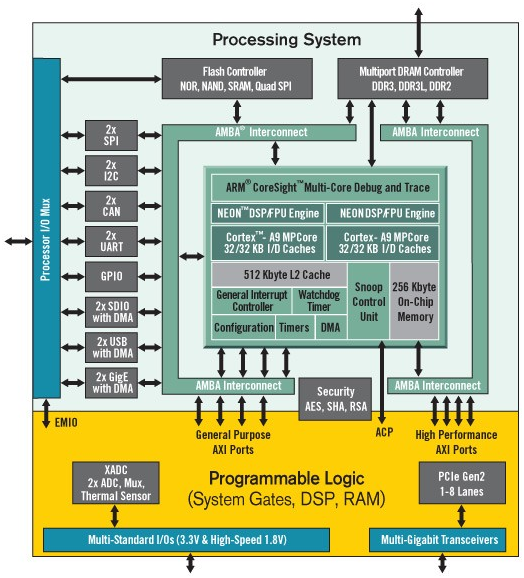
\includegraphics[width=\textwidth]{zynq.png}
	\caption{Architektura układu Zynq SoC \cite{zynq}.}
	\label{fig:zynq}
\end{figure}
%TODO Coś o kamerze, ale parametry. Te szczegóły techniczne to przy implementacji
\section{Moduł rejestrujący obraz}
\label{sec:pcam}
W~projekcie wykorzystano kolorową kamerę Digilent~PCAM~5C. Jest to~moduł przeznaczony do~użycia z~dedykowanymi płytkami rozwojowymi. Jednym z~kompatybilnych układów jest ZYBO Z7-20. Właściwości modułu przedstawiono poniżej:
\begin{itemize}
	\item Rozdzielczość: 5 MPx,
	\item Matryca: OV5640,
	\item Interfejs danych: MIPI CSI-2
	\item Złącze: 15-pinowe FFC
\end{itemize}
Sposób podłączenia kamery i~układu ZYBO Z7-20 przedstawione zostaly w~sekcji \ref{sec:integracja_uklad_kamera}.
\section{Platforma statku powietrznego}
\label{sec:platforma_statku_powietrznego}
Zdecydowano się na~dron sześciowirnikowy, znajdujący się na~wyposażeniu studenckiego koła naukowego AVADER. Zbudowanie drona było częścią innego projektu \cite{mgr}. Elementy użytego bezzałogowago statku powietrznego to:
\begin{itemize}
	\item rama DJI F550,
	\item śmigła o średnicy równej 22,86~cm oraz skoku 12,7~cm,
	\item silniki DJI 2312/960KV z kontrolerami 420 LITE,
	\item czterokomorowa bateria LiPo o nominalnym napięciu 14,8~V i~pojemności 6450mAh, 
	\item nadajnik radiowy FrSky Taranis X9D Plus, odbiornik FrSky X8D,
	\item sterownik 3DR Pixhawk.
\end{itemize}
\section{Autopilot}
\label{sec:autopilot}
Urządzeniem bezpośrednio komunikującym się z~kontrolerami silników drona jest autopilot. W~pracy wykorzystano sterownik Pixhawk, będący popularnym kontrolerem lotu ogólnego przeznaczenia dostępnym na~otwartej licencji.
Jego główne parametry~to:
\begin{itemize}
	\item procesor Cortex-M4F z zegarem 168 MHz,
	\item czujniki: akcelerometr, żyroskop, kompas magnetyczny, barometr i~zewnętrzny moduł GPS,
	\item interfejsy: UART, CAN, I2C, SPI,
	\item wejście karty SD,
	\item zewnętrzny przełącznik bezpieczeństwa uzbrajania,
	\item wielokolorowa dioda pokazująca stan pracy
\end{itemize}
Konfiguracja sterownika jest możliwa przy użyciu programu Mission Planner. Jest to~aplikacja przeznaczona dla~stacji naziemnej umożliwiająca:
\begin{itemize}
	\item strojenie czujników autopilota,
	\item monitorowanie stanu sterownika (uzbrojenie silników, orientacja statku powietrznego),
	\item planowanie, zapisywanie i~wgrywanie planów autonomicznych misji statku powietrznego,
	\item pobieranie i~analizowanie dzienników misji.
\end{itemize}
Sterownik umożliwia pracę w~różnych trybach.
W~zależności od~aktywnego tybu, zadania wykonywane przez autopilota nieco się różnią. Z~punktu widzenia autonomicznego lotu, najbardziej interesującym trybem jest tryb GUIDED. Umożliwia on~bowiem wydawanie dronowi poleceń. Zazwyczaj komunikacja przebiega drogą radiową ze~stacją naziemną (przy użyciu programu Mission Planner), lecz wysyłanie komend przez urządzenie umieszczone na~platformie drona również jest możliwe.

Kwestię połączenia autopilota i układu ZYBO Z7-20 opisano w sekcji \ref{sec:integracja_plytka_autopilot}.